%%% LyX 2.0.5.1 created this file.  For more info, see http://www.lyx.org/.
%% Do not edit unless you really know what you are doing.
%\documentclass[english]{report}
%\usepackage[T1]{fontenc}
%\usepackage[latin9]{inputenc}
%\setcounter{secnumdepth}{3}
%\setcounter{tocdepth}{3}
%\usepackage{setspace}
%\onehalfspacing
%\usepackage{babel}
%\usepackage{verbatim}
%\usepackage{pdfpages}
%\usepackage{graphicx}
%\usepackage{subfig} %% This package has to be here
%\usepackage{setspace}
%\usepackage{arabtex}
%\usepackage[numbers]{natbib}
%\usepackage{nomencl}
%\usepackage{amsthm}
%\usepackage{bbold}
%
%\makenomenclature
%
%% Theorem Styles
%\newtheorem{theorem}{Theorem}[section]
%\newtheorem{lemma}[theorem]{Lemma}
%\newtheorem{proposition}[theorem]{Proposition}
%\newtheorem{corollary}[theorem]{Corollary}
%% Definition Styles
%\theoremstyle{definition}
%\newtheorem{definition}{Definition}[section]
%\newtheorem{example}{Example}[section]
%\theoremstyle{remark}
%\newtheorem{remark}{Remark}
%
%\begin{document}

\chapter{Data Collection}
\label{chap:samples_collection}

The data is the most important part ofearning technique. 
The quality of the collected data and it's amount is a fundamental

Thus, the data collection stage is an important stage in the development of our system. The Arabic alphabet consists of 29 isolated characters. If we ignore all diacritical marks, which do not carry important information about shape, we obtain 18 shapes.

\begin{figure}
\centering
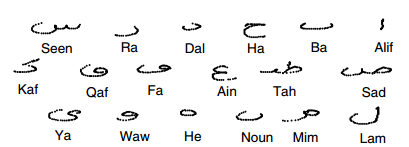
\includegraphics{./figures/arabic_letters}       
\caption{The set of all distinctive main body Arabic letters.}
\label{fig:arabic_letters}
\end{figure}

The writing of these characters was not constrained, leading to a wide variety of size, and orientation. Figure (5) shows some samples of the "Ha" letter written by several writers.

\begin{figure}
\centering
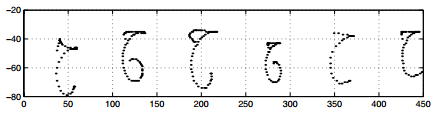
\includegraphics{./figures/ha_different}       
\caption{Different writing styles of the isolated form of the letter \RL{h} (Ha)}
\label{fig:ha_different}
\end{figure}

We utilize two sources of letters samples written in different positions and different types of writing. The first is a self-made database of letters that were collected from different age Arabic writers using digitizer tablet. We discuss these two methods in more details below. In both cases the information is a sequence $\pi=[p_1,...,p_n]$ where the vector $p_i=(x_i,y_i)$ denotes the horizontal and vertical coordinates, sampled from the writer's pen movement.

\section{A self-collected letters database}
We have developed an application, using Matlab, which asks the user to draw a letter on an electronic pad, the $(x,y)$ sequence data of the letter shape was saved as a file on the file system.  The rectangle in which the user was asked to draw the letter is $1\times1$. See image of the GUI below. \emph{[Add an Image of the Matlab data collection UI]}. 

\section{Letters Extraction from the ADAB Database}
The other source was the ADAB database. The ADAB contains Arabic script samples. The information saved is the strokes information; each stroke contains the sequence of $(x,y)$ coordinates of the pen down to pen up. The challenge was to match each word part to each stroke, and then manually segment each sequence which describes a word-part to letters (subsequences). Another problem we faced was that automatically corresponding each stroke o each word-part was not easy. \emph{[talk more abour it - Wajdi]}


\section{The ADAB Database}

\section{Letters Extraction}
\begin{itemize}
\item Discuss the letters extraction from the adab database.
\item Describe the system developed by Wajdi
\item mention that the number of samples per class is different from letter to letter
\end{itemize}

\subsection{Additional strokes detection and removal}
\emph{TODO: talk about the the need to remove additional strokes. that our thesis considers only the main body. and that there are letters that can be identified only by the additional strokes like \RL{r,z} and that there are combination of letters that may look like othger letter like double \RL{b} and \RL{s}} 

\emph{see "Removing delayed strokes" section in  \cite{jaeger2001online}}

{\color{blue}The detection of delayed strokes is performed based on
their sequential order, location, and size. Delayed strokes
are detected based on the size and shape of their bounding
box with respect to the word-part.\cite{saabni2009hierarchical}}

\section{Data representation Definition}
On-line handwriting data is commonly a digitized representation of the pen movement. It may contain sequential information about position, velocity, acceleration, pressure, or even angle and orientation of the pen as a function of time. However, the most basic and used property is the position of the pen. In addition, usually in HWR systems the pen position is not given as a function of time, but as an ordered set of sequential pen position. 

A formal definition of the representation of pen position acquired data, the stroke, is given as follows: 
\begin{definition}
A stroke $S$ is defined as a sequence points in the two-dimensional space and given as follows:
\begin{equation}
S = \left[(x_1,y_1),...,(x_N,y_N)\right]
\end{equation} 
where N is the number of samples in the stroke. 
\end{definition}

Let us denote the stroke space of all lengths as $D$ and the space that contains strokes of length $N$ as $D^N$. 

\section{Letters samples statistics}
number of samples per letter and letter position.
number of samples used to extract the letters

%\end{document}
